% Questions on PDF page 134
\documentclass[11pt]{article}

\usepackage[utf8]{inputenc}
\usepackage[a4paper, margin=.9in]{geometry}
\usepackage{booktabs}
\usepackage{enumerate}
\usepackage{enumitem}
\usepackage{physics}
\usepackage{amsmath}
\usepackage{amsfonts}
\usepackage{graphicx}
\usepackage{siunitx}
\usepackage{textcomp}
\usepackage{hyperref}

\bibliographystyle{ieeetr}
\graphicspath{{./figures}}

\title{Big Data (AES 690) Project Proposal}
\author{Mitchell Dodson}
\date{March 8, 2024}

\newcommand*{\problem}[2]{
    \begin{table}[ht]
    \centering
        \begin{tabular}{ | p{.1\linewidth} p{.9\linewidth} | }
            \hline
            \vspace{.3em}\textbf{\large#1:} & \vspace{.3em}\small{#2}\hspace{.2em}\vspace{.5em} \\ \hline
        \end{tabular}
    \end{table}
}

\begin{document}

\maketitle

\newpage

\begin{figure}[h!]
    \centering

    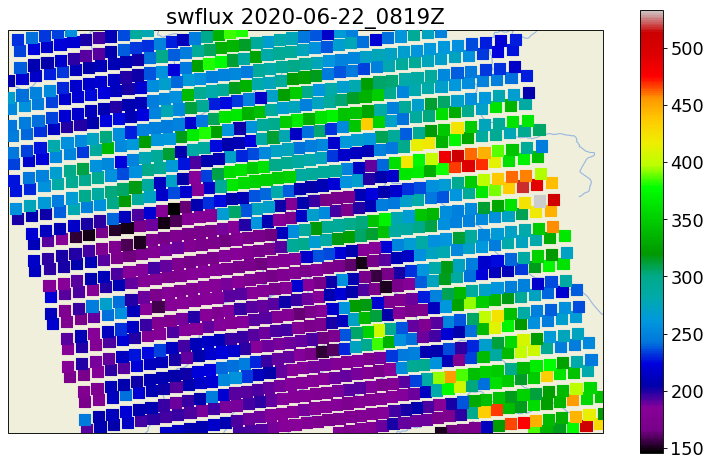
\includegraphics[width=.33\linewidth]{figs/geo_scatter_2020-06-22_0819Z_swflux.png}
    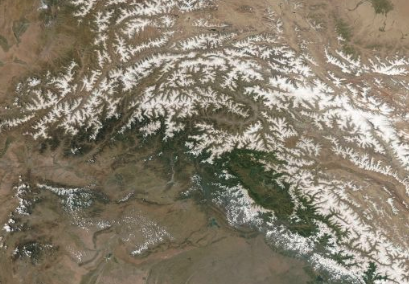
\includegraphics[width=.31\linewidth]{figs/20200622_0819_hkh_modis.png}
    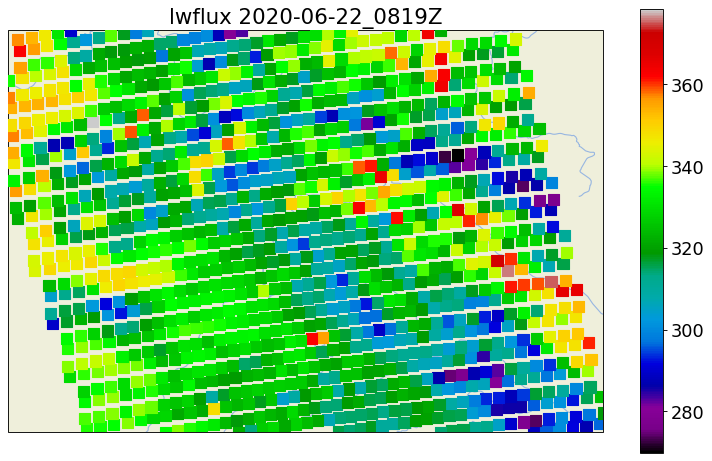
\includegraphics[width=.33\linewidth]{figs/geo_scatter_2020-06-22_0819Z_lwflux.png}

    \caption{Comparison between the CERES shortwave flux (left), coincident MODIS image (middle), and CERES longwave flux (right). Captured by Aqua over the Hindu Kush Himalayan region on June 22, 2020 at 0819Z. Note the contrast between cold and bright mountaintop snow, warm dark vegetation, and warm bright desert surfaces.}
    \label{ceres_modis_compare}
\end{figure}

\noindent
{\large\textbf{Abstract}}

Our modern understanding of Earth's energy budget relies heavily on the direct observation of outgoing radiance by polar-orbiting satellites. Space-based platforms like the Earth Observation System (EOS) Terra and Aqua satellites are indispensable for characterizing the governing processes and magnitudes of fluxes leaving Earth's surface and atmosphere since they have frequent global coverage and offer direct measurement of the outgoing energy at the top of a full atmospheric column. Nonetheless, broad-band bolometers like EOS' Clouds and Earth's Radiant Energy System (CERES) are limited in that they generally have coarse spatial resolutions, and the conversion from the observed directional radiance to an estimate of full-sky flux depends on Angular Distribution Models (ADMs), which themselves require simultaneous data from finer-resolution narrow-band radiometers like EOS' Moderate Resolution Imaging Spectroradiometer (MODIS). In order to address both of these shortcomings, I propose a novel machine learning methodology with the potential to (1) emulate the ADMs in order to predict the coarse longwave and shortwave fluxes from CERES given only MODIS pixels and viewing geometry, and (2) sharpen the fluxes to the MODIS resolution.

\vspace{1em}

\noindent
{\large\textbf{Background}}

The utility of satellites for building a holistic picture of Earth's outgoing radiation has been understood since the dawn of the space age. The earliest satellite-derived estimates of Earth's overall albedo (30\%) and emission temperature ($253\,\si{K}$) were acquired from the TIROS-generation satellites in the mid-1960s, and later improved by the ESSA III platforms into the 1970s \cite{haar_measurements_1971}\cite{suomi_theoretical_1967}. One major challenge became quickly apparent: the quantity of interest is the full-sky \textit{flux} ($\si{W.m^{-2}}$) exiting the hemisphere above a surface, but the bolometers can only ever observe directional \textit{radiance} ($\si{W.m^{-2}.sr^{-1}}$) from a surface into the aperture. Many surfaces are highly anisotropic, so assuming they uniformly radiate the observed amount of energy in every direction is erroneous. The next generation of broad-band radiometers were launched aboard Nimbus-7, NOAA-10, and NOAA-11 in the 1970s as part of the Earth's Radiation Budget Experiment (ERBE) program. These satellite platforms also host Advanced Very High Resolution Radometer (AVHRR) narrow-band sensors which provide enough spectral information to group surfaces into categories with similar anisotropy models \cite{ramanathan_cloud-radiative_1989}\cite{smith_inversion_1986}.

The EOS satellites continued with this approach by carrying CERES and MODIS sensors, which have a data record of about 25 years. CERES has a sub-satellite instantaneous field of view (hereafter \textit{footprint}) of about $16\times 32 \,\si{km}$, and MODIS has a $~1\,\si{km}$ pixel resolution, so many MODIS pixels can be directly co-located within each CERES footprint. During the L2 preprocessing of CERES SSF data, the MODIS data are used to identify land surfaces, mask water, and derive cloud and aerosol properties. Once a category is determined for each pixel in a footprint, the corresponding ADMs are selected and evaluated for the viewing geometry, and their returned anisotropy factors are combined by weighted sum according to the CERES point spread function (PSF). The subsequent aggregated anisotropy factor is the value used to convert the footprint's radiance observed by CERES to the full-sky flux estimates included in the CERES SSF product \cite{loeb_earths_2018}. In the past 40 years, considerable attention has been directed towards identifying clusters in surface types' angular dependence \cite{suttles_angular_1988}, and developing associated ADMs that are carefully-validated with respect to ground station data and specialized satellite sensors like EOS' Multi-angle Imaging SpectroRadiometer (MISR) \cite{loeb_defining_2002} \cite{su_next-generation_2015}.

\begin{figure}[h!]
    \centering

    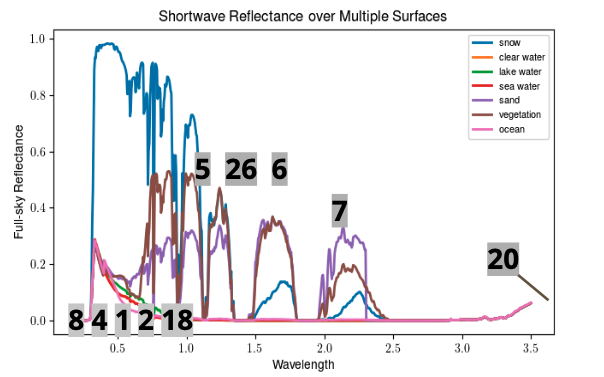
\includegraphics[width=.48\linewidth]{figs/sbdart_sw.png}
    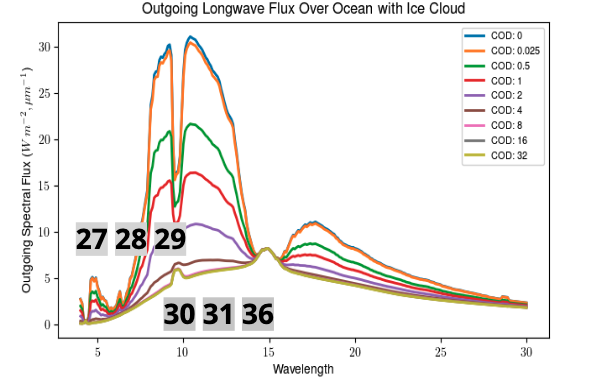
\includegraphics[width=.48\linewidth]{figs/sbdart_lw.png}

    \caption{Comparison of top-of-atmosphere outgoing spectral flux of multiple surfaces in the shortwave and longwave ranges, with several MODIS bands' center wavelegnths approximately labeled. CERES effectively observes the area under each spectral curve, and MODIS pixels may be considered point data at the specific wavelengths. Data were generated with SBDART \cite{ricchiazzi_sbdart_1998}.}
    \label{ceres_modis_compare}
\end{figure}

\noindent
{\large\textbf{Hypothesis}}

The full-sky fluxes inverted from broad-band CERES radiances by modern ADMs have been well-validated, but flux estimates still intermediately rely on sophisticated cloud and aerosol property retrievals and annualized discrete surface classes to pick an anisotropy model. Since the cloud properties and surface classes informing ADMs are derived from MODIS radiance data, the information needed to determine surface characteristics should be available in the pixel’s spectral properties.

In fact, since MODIS pixels include narrow bands that are intentionally centered at salient wavelengths throughout most of the solar and terrestrial emission spectra, the spectral response of a collection of MODIS pixels within a CERES footprint may be able to directly predict the well-validated full-sky longwave and shortwave fluxes of the footprint. In particular, reflected solar irradiance in the $.45-3.6\,\si{\mu m}$ range is measured by 21 shortwave bands including visible bands that help characterize color and albedo, near infrared bands that distinguish vegetation, surface water, hydrometeor phase, and particle size, and shortwave infrared bands for fires and emissivity. Furthermore, terrestrial emissions in the $3.6-14.4\,\si{\mu m}$ range are captured by 16 longwave infrared bands, which help characterize atmospheric O$_3$ and CO$_2$ content, surface temperatures, and the distribution of water vapor in the atmosphere.

As such, my primary hypothesis is that a neural network trained on MODIS pixels can learn to predict the full-sky flux values of CERES SSF footprints over multiple surfaces and viewing geometry configurations. If the above model is performant, my secondary hypothesis is that an additional network module can be trained to estimate longwave and shortwave flux at the MODIS 1km resolution.

\vspace{1em}

\noindent
{\large\textbf{Methodology}}

The model starts with an encoder producing a grid of latent vector embeddings by applying the same weights independently to each MODIS pixel. This may be thought of as a dimensionality reduction technique encouraging the model to find a condensed latent representation of information about each pixel's surface and radiative properties. Next, the latent outputs are aggregated by a weighted sum according to the CERES point spread function, which adjusts the contribution of each latent vector in the footprint to the spatial sensitivity of the CERES instrument. The aggregated latent vector is then concatenated with the footprint viewing geometry and passed to a decoder. The decoder component of the model serves to emulate the ADM, using the distilled and aggregated information on radiative and surface properties from MODIS in combination with the whole scene's viewing geometry (solar zenith, viewing zenith, and relative azimuth) to estimate the CERES-observed shortwave and longwave full-sky fluxes.

If this approach is successful, I will extend the model to predict the flux contribution of each MODIS pixel. With the viewing geometry and the full latent grid as inputs, the extended model will impose the aggregate flux estimates from the previous model as a constraint on the PSF-weighted sum of its predictions in the loss function. It will be interesting to investigate the pixel-wise information encoded in each vector of the latent grid, and to experiment with the consequences of modulating the viewing geometry while holding the vector constant. It's also worth noting that since the encoder applies the same weights independently to each MODIS pixel, and since the latent pixels are aggregated by a simple weighted sum, the trained network will be agnostic toward the number or spatial properties of the input pixels.

\begin{figure}[h!]
    \centering

    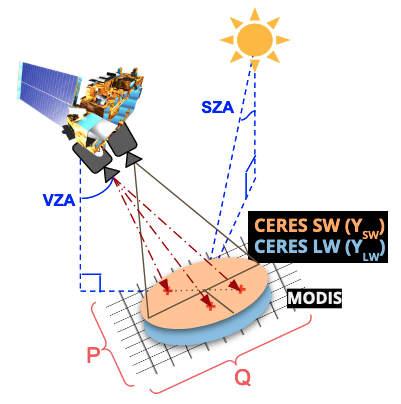
\includegraphics[width=.38\linewidth]{figs/sat_schematic.png}
    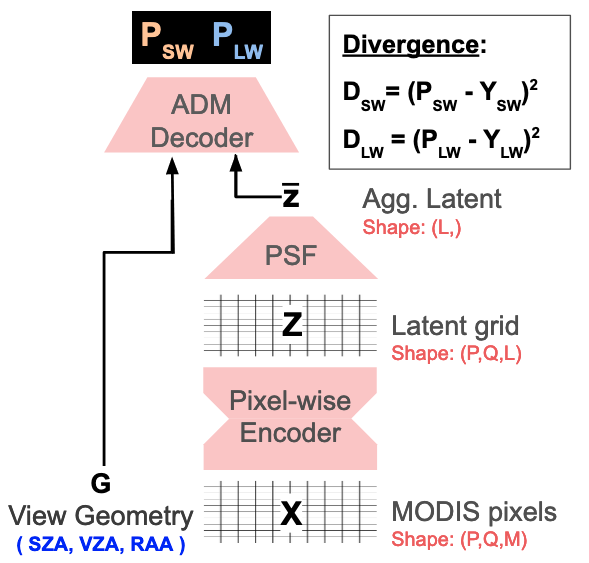
\includegraphics[width=.38\linewidth]{figs/model_arch.png}

    \caption{Schematic diagrams of the sun/pixel/sensors system and aggregate flux predictor architecture. The model applies the same weights to each size M pixel on the (P,Q) shaped grid, and generates a size L latent vector for each. The subsequent (P,Q,L) shaped grid is aggregated to a single size L latent vector by the PSF, then concatenated with the 3-element viewing geometry. Finally, a feedforward decoder takes the size L+3 combined vector as input, and tries to predict the CERES-observed longwave and shortwave flux.}
    \label{schematic}
\end{figure}


\noindent
{\large\textbf{Development Agenda}}

\vspace{-1em}

\begin{enumerate}[itemsep=0pt, parsep=0pt, before=\setlength{\baselineskip}{6mm}]
    \item Acquire multiple years of EOS satellite overpasses within several small regions selected to have a wide variety of surface types and overpass times. Calculate the satellite-relative viewing angles for both datasets, and save the MODIS subgrid, CERES footprints, and geometric information for each overpass as an HDF5 file identified by its region and capture time.
    \item Create a TensorFlow Dataset generator that selects CERES footprints, extracts their MODIS subgrids, and calculates the point spread function over each subgrid. The generator must open multiple overpass HDF5 files in separate processes and interleave their data in order to support training generalization.
    \item Train the above architecture with a variety of hyperparameters such as network width, layer count, activation and, crucially, latent vector size. Attempt latent variational distribution.
    \item Test the robustness of the model's flux predictions by modulating the viewing geometry, inputs, and latent values. Verify that the predictions remain physically realistic.
\end{enumerate}



\newpage

\bibliography{main}

\end{document}

\begin{figure}[h!]
    \centering

    \includegraphics[width=.6\paperwidth]{}

    \caption{}
    \label{f1}
\end{figure}


\begin{figure}[h!]\label{q1q2}
    \centering
    \begin{tabular}{ c c c | c}
    \end{tabular}
\end{figure}

